\chapter{Oprogramowanie}

Do rozwiązania opisanego w poprzednim rozdziale problemu skonstruowano i zaimplementowano dwa algorytmy: dokładny oraz przybliżony.
Ze względu na to, że problem przepływowy jest NP-trudny, często rezygnuje się z algorytmów dokładnych. Powodem takiego stanu rzeczy jest wykłądnicza złożoność obliczeniowa. Rozpatrywany w prac problem jest pewnym uogólnieniem problemu przepływowego, jest więc także NP-trudny.

W przedstawionym przypadku użyty został algorytm dokładny (przegląd zupełny), ponieważ liczba zadań jest niewielka oraz planowanie w systemie jest offline (nie ma ograniczeń czasowych na uzyskanie rozwiązania).
W celu porównania wybrano algorytm metaheurystyczny (symulowane wyżarzanie), który nie daje rozwiązania optymalnego, lecz dostatecznie dobre w krótkim czasie. Będzie on stosowany w przypadku produkcji większej liczby płytek.

\section{Implementacja}
Algorytm zaimplementowano w języku C++ przy wykorzystaniu środowiska Qt. Jest to zestaw darmowych narzędzi i bibliotek, służących do tworzenia aplikacji okienkowych oraz konsolowych. Niewątpliwą zaletą Qt jest jego wieloplatformowość, dzięki czemu przy użyciu jednego kodu bazowego, może on być zaimplementowany w różnych środowiskach (Windows, Linux, macOS, Android oraz systemy wbudowane).

Przykład działania programu na Rysunku~\ref{app_out}

\begin{figure}[H]
	\centering
	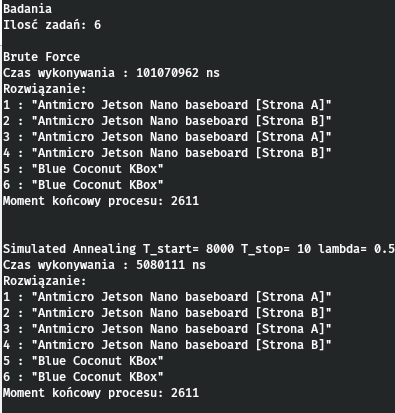
\includegraphics[scale=0.6]{chapters/chapter4/app_out.png}
	\caption{Wyjście programu.}
	\label{app_out}
\end{figure}

\breakparagraph{}
W celu łatwego i usystematyzowanego dostępu do informacji o poszczególnych projektach i czasach wykonywania, zaprojektowano i stworzono bazę danych. Zastosowany został system zarządzania bazą danych SQLite.

\breakparagraph{}
Zalety SQLite:
\begin{itemize}
	\item rozwiązanie wieloplatformowe,
	\item cała baza danych to tylko jeden plik,
	\item duża zgodność z standardem SQL,
	\item duża wydajność (silnik napisany w języku C).
\end{itemize}

\paragraph{}
Projekt bazy danych składa się z trzech tabel (Rysunek~\ref{baza_danych}):
\begin{itemize}
	\item projects --- tabela zawierające podstawowe informacje o poszczególnych projektach,
	\item operation\_time --- tabela zawierająca czasy trwania poszczególnych operacji per projekt,
	\item changeover\_time --- tabela zawierająca czasy przezbrojenia poszczególnych projektów.
\end{itemize}

\begin{figure}[H]
	\centering
	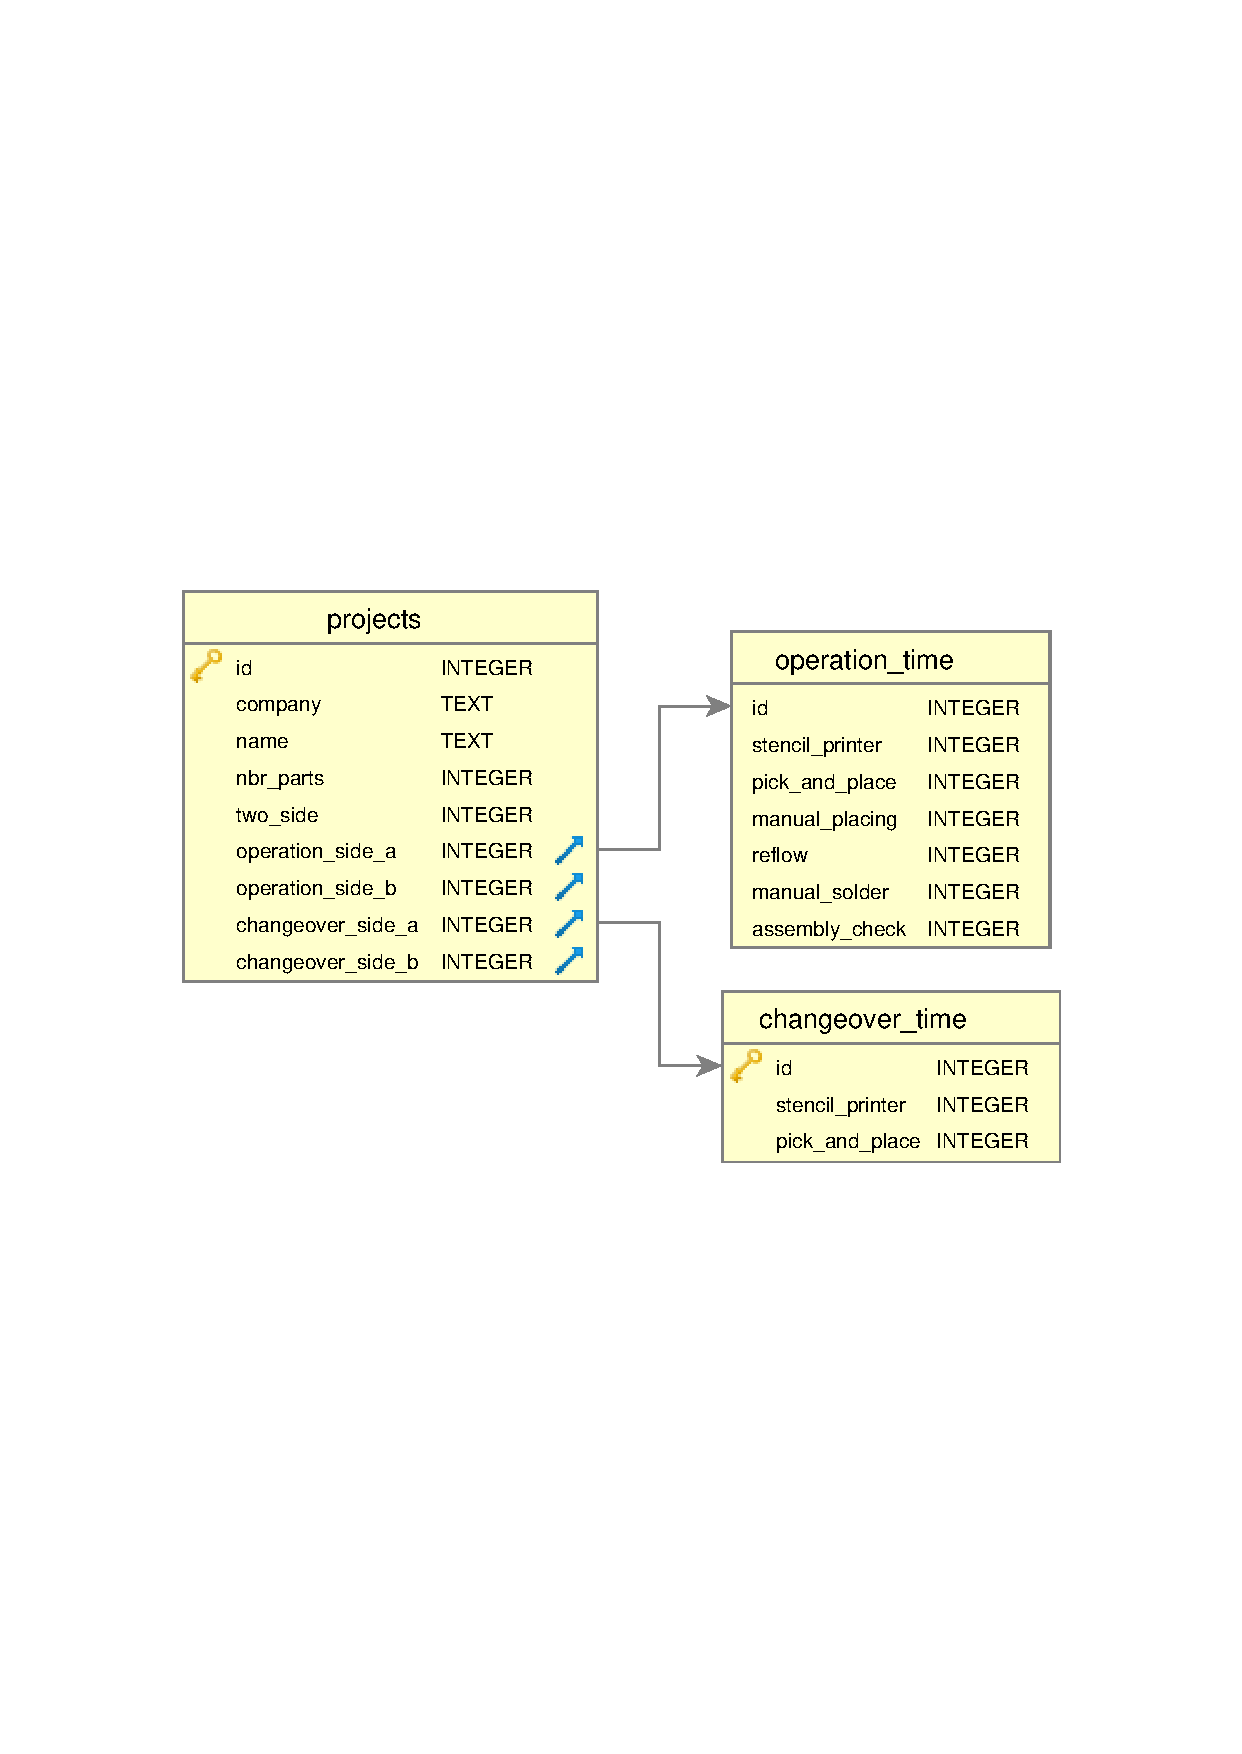
\includegraphics[scale=0.9]{chapters/chapter4/db_crop.pdf}
	\caption{Struktura bazy danych}
	\label{baza_danych}
\end{figure}


Opis poszczególnych pól struktur baz danych został przedstawiony w Tabelach~\ref{projects}--\ref{oper}.

\begin{table}[H]
	\centering
	\caption{Opis pól w tabeli ``projects''}
	\begin{tabular}{lll}
		\toprule
		Pole tabeli         & Opis                                    & Format pola       \\
		\midrule
		id                  & Indeks projektu                         & Liczba całkowita \\
		company             & Nazwa firmy                             & Tekst             \\
		name                & Nazwa projektu                          & Tekst             \\
		nbr\_parts          & Ilość elementów                      & Liczba całkowita \\
		two\_side           & Czy płyta posiada 2 warstwy            & Liczba całkowita \\
		operation\_side\_a  & Indeks do czasów operacji dla strony A & Liczba całkowita \\
		operation\_side\_b  & Indeks do czasów operacji dla strony B & Liczba całkowita \\
		changeover\_side\_a & Indeks do czasów przezbrojenia         & Liczba całkowita \\
		changeover\_side\_b & Indeks do czasów przezbrojenia         & Liczba całkowita \\
		\bottomrule
	\end{tabular}
	\label{projects}
\end{table}

\begin{table}[H]
	\centering
	\caption{Opis pól w tabeli ``changeover\_time''}
	\begin{tabular}{lll}
		\toprule
		Pole tabeli      & Opis                              & Format pola       \\
		\midrule
		id               & Indeks rekordu                    & Liczba całkowita \\
		stencil\_printer & Czas przezbrojenia na sitodruku   & Liczba całkowita \\
		pick\_and\_place & Czas przezbrojenia na pick\&place & Liczba całkowita \\
		\bottomrule
	\end{tabular}
	\label{changeover}
\end{table}

\begin{table}[H]
	\centering
	\caption{Opis pól w tabeli ``operation\_time''}
	\begin{tabular}{lll}
		\toprule
		Pole tabeli      & Opis                                          & Format pola       \\
		\midrule
		id               & Indeks rekordu                                & Liczba całkowita \\
		stencil\_printer & Czas operacji na sitodruku                    & Liczba całkowita \\
		pick\_and\_place & Czas operacji na pick\&place                  & Liczba całkowita \\
		manual\_placing  & Czas operacji ręcznego nakładani elementów & Liczba całkowita \\
		reflow           & Czas operacji lutowania w piecu               & Liczba całkowita \\
		manual\_solder   & Czas operacji ręcznego lutowania             & Liczba całkowita \\
		assembly\_check  & Czas operacji kontroli wizualnej              & Liczba całkowita \\
		\bottomrule
	\end{tabular}
	\label{oper}
\end{table}

Dane wprowadzone zostały do bazy danych przy pomocy aplikacji DataGrip. Na rysunkach~\ref{dg:proj}--\ref{dg:changeover} przedstawiono tą operację dla każdej tabeli.

\begin{figure}[H]
	\centering
	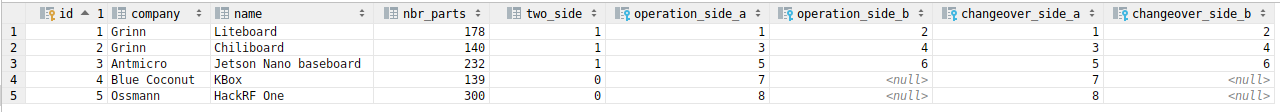
\includegraphics[width=\linewidth]{chapters/chapter4/projects_db.png}
	\caption{Tabela ``projects'' w DataGrip}
	\label{dg:proj}
\end{figure}

\begin{figure}[H]
	\centering
	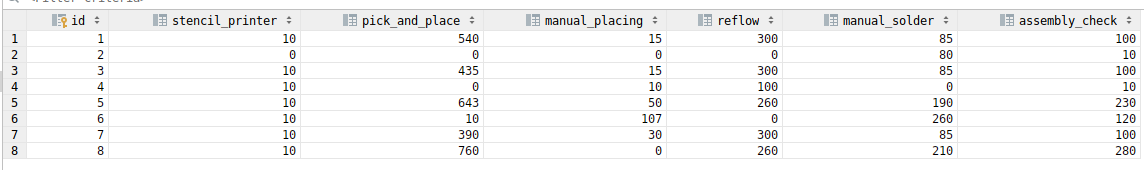
\includegraphics[width=\linewidth]{chapters/chapter4/opera_db.png}
	\caption{Tabela ``operation\_time'' w DataGrip}
	\label{dg:oper}
\end{figure}

\begin{figure}[H]
	\centering
	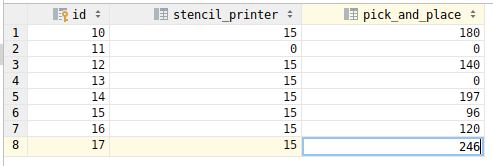
\includegraphics[scale=0.9]{chapters/chapter4/changeover_db.png}
	\caption{Tabela ``changeover\_time'' w DataGrip}
	\label{dg:changeover}
\end{figure}

\section{Przegląd zupełny}

Przegląd zupełny (ang. Brute-force search) jest to algorytm polegający na wyznaczeniu wszystkich możliwych permutacji zadań (rozwiązań dopuszczalnych), a następnie wybraniu z tego zbioru najlepszego rozwiązania. Jest to algorytm dokładny, przez co rozwiązanie jest zawsze optymalne, lecz niestety okupione dużą czasochłonnością obliczeń.

Diagram na Rysunku~\ref{brute_force} przedstawia ideę algorytmu. W celu wygenerowania wszystkich permutacji zadań, wykorzystano algorytm porządku leksykograficznego (Rysunek~\ref{gen_perm}).

\section{Metoda symulowanego wyżarzania}
Symulowane wyżarzanie (ang. Simulated annealing,w skrócie SA) to kombinatoryczna metoda optymalizacji oparta na szukaniu losowo rozwiązania~\cite{sa}. Algorytm ten jest oparty na analogii pomiędzy zjawiskiem wyżarzania metali, a optymalizacją złożonych problemów kombinatorycznych. Wiele tych problemów jest NP-trudnych, co powoduje, że istnienie algorytmów dokładnych, o wielomianowym czasie obliczeniowym, jest niemożliwe. Symulowane wyżarzanie jest zatem idealnym wyborem, ze względu na jego elastyczność, szybkość działania oraz jakość rozwiązań, przez co nie ma ograniczeń przy doborze do problemu.

Cechą która odróżnia metodę symulowanego wyżarzania od innych metod metaheurystyczny to używanie funkcji akceptacji. Funkcja akceptacji pozwala na opuszczanie ekstremum lokalnego przez przyjęcie chwilowo gorszego rozwiązania. Wzór na funkcję akceptacji:
\begin{equation}
	p=exp(\frac{F(x')-F(x)}{T}),
\end{equation}

gdzie:
\begin{itemize}
	\item $T$ --- bieżąca temperatura,
	\item $x'$ --- nowe wygenerowane rozwiązanie,
	\item $x$ --- rozwiązanie bazowe
\end{itemize}

W algorytmie SA istotną rolę odgrywają: dobór odpowiednich parametrów, strategii schładzania oraz dobranie techniki ruchu po przestrzeni (generowanie otoczeń).

\breakparagraph{}
Symulowane wyżarzanie posiada 3 parametry wpływające na jego działanie:
\begin{itemize}
	\item $T_{start}$ --- temperatura początkowa (wartość początkowa temperatury),
	\item $T_{stop}$ --- temperatura końcowa (ewentualny warunek stopu),
	\item $\lambda$ --- współczynnik schładzania (tempo, w jakim temperatura ma spadać).
\end{itemize}

\breakparagraph{}
Stosuję się najczęściej dwa schematy schładzania~\cite{Smutnicki2002As}:
\begin{itemize}
	\item geometryczny $T = \lambda T$
	\item logarytmiczny $T = T /(1 + \lambda T)$
\end{itemize}

\breakparagraph{}
Wybór strategii schładzania zależy w dużej mierze od problemu, jaki będzie rozwiązywany przez algorytmem.

\breakparagraph{}
W metodzie symulowanego wyżarzania tak jak w wielu innych metaheurystykach ważny jest wybór techniki generowania otoczeń. Najpopularniejsze z nich to:
\begin{itemize}
	\item zamień --- wybranie dwóch losowych elementów i ich zamiana miejscami,
	\item zamień sąsiednie --- wybranie losowego zadania, a następnie zamiana kolejności z następnym zadaniem na liście,
	\item wstaw --- wybranie losowego elementu, który przesuwamy na losową pozycję na liście.
\end{itemize}


\breakparagraph{}
W pracy zaimplementowano podstawową wersję algorytmu (Rysunek~\ref{sa}).
\raggedbottom{}


\section{Diagramy}
\begin{figure}[H]
	\centering
	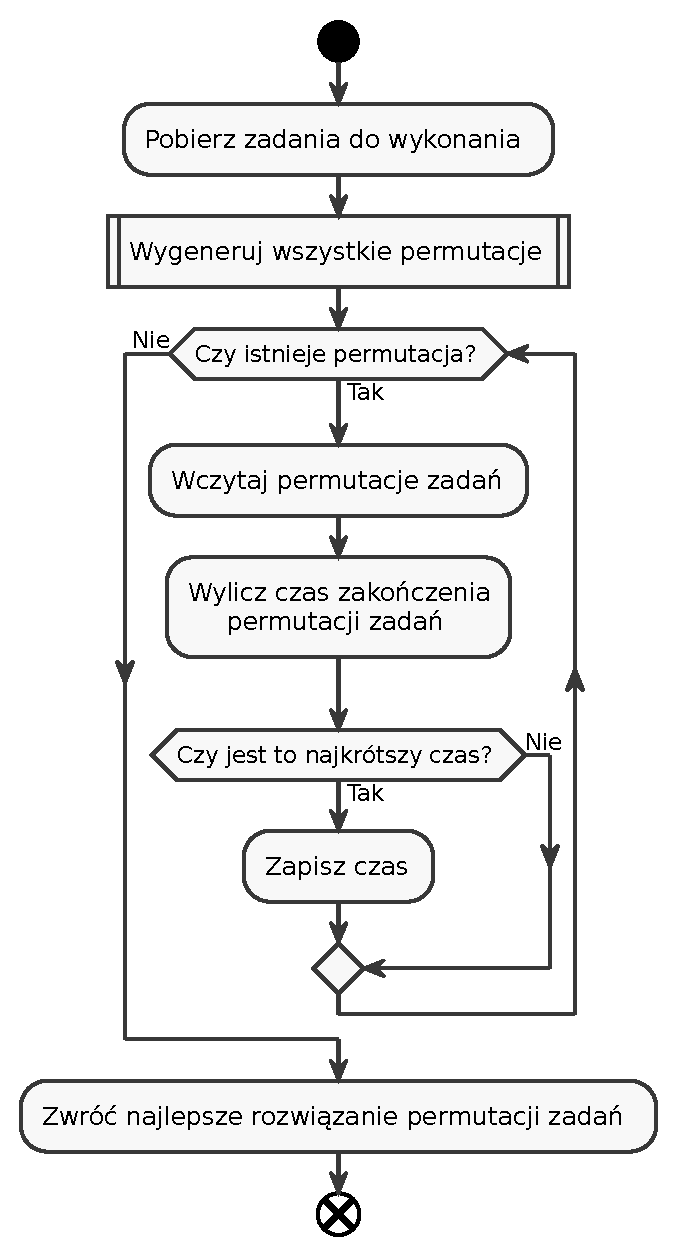
\includegraphics[scale=0.65]{chapters/chapter4/brute_force.pdf}
	\caption{Diagram algorytmu ``Przegląd zupełny''}
	\label{brute_force}
\end{figure}

\begin{figure}[H]
	\centering
	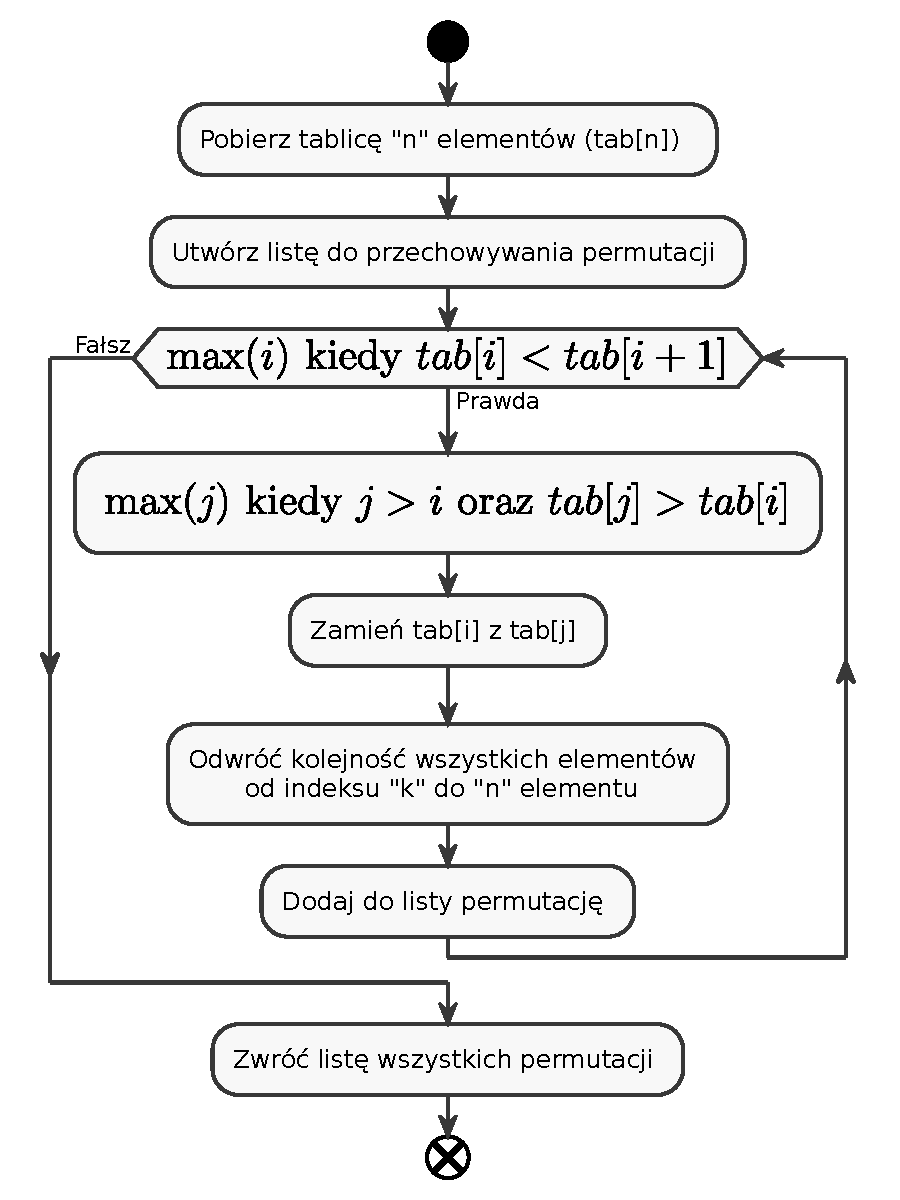
\includegraphics[]{chapters/chapter4/gen_perm.pdf}
	\caption{Diagram algorytmu ``Porządek leksykograficzny''}
	\label{gen_perm}
\end{figure}



\begin{figure}[H]
	\centering
	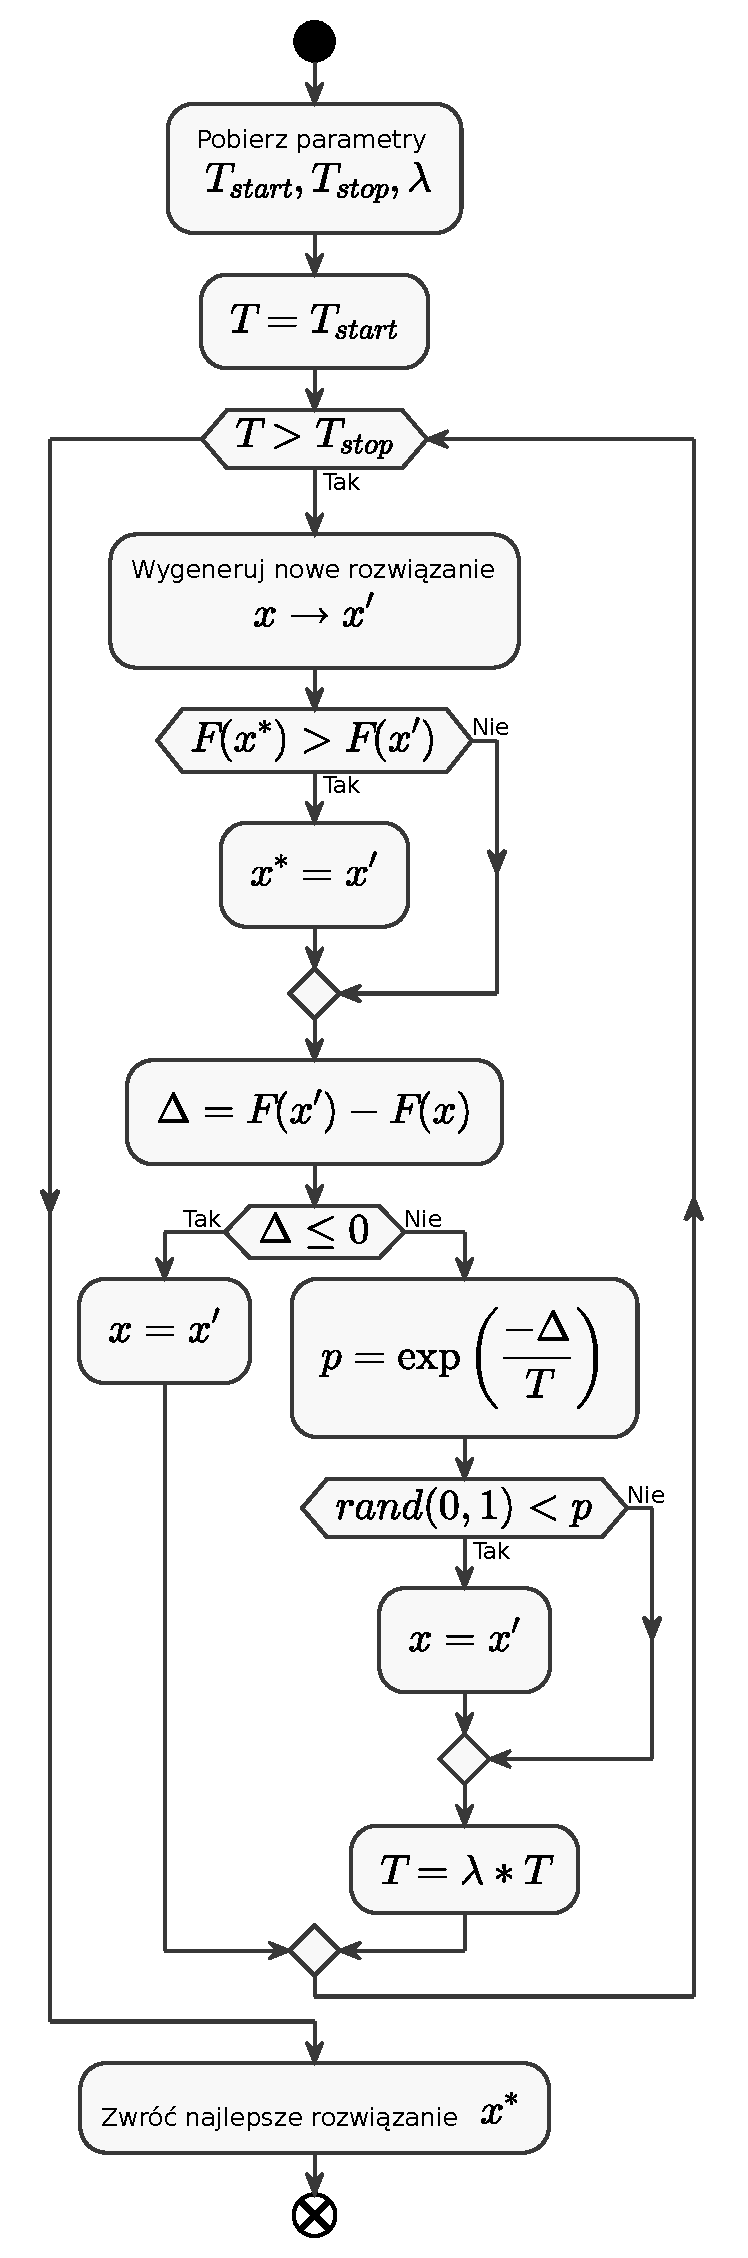
\includegraphics[scale=0.67]{chapters/chapter4/sa.pdf}
	\caption{Diagram algorytmu ``Symulowane wyżarzanie''}
	\label{sa}
\end{figure}
